\documentclass[11pt,a4paper]{article}
\usepackage{fontspec}
\usepackage{xeCJK}
\xeCJKsetup{CJKspace=true}
\setCJKmainfont{Apple SD Gothic Neo}
\setmainfont{Times New Roman}
\usepackage{amsmath,amssymb,bm}
\usepackage{booktabs}
\usepackage{graphicx}
\graphicspath{{simulation/}}
\usepackage{geometry}
\geometry{margin=2.3cm}
\usepackage[hidelinks]{hyperref}
\usepackage{caption}
\captionsetup{font=small}

\title{\textbf{L4 리스크 카드 통합의 방법론과 실증 결과}\\[4pt]
\large Multi-Resolution Dendrogram, 생성형 명명·2인 검수, 원천 손상 교정을 포함한 통합 기술 보고서 v2}
\author{천영삼 (Responsible AI, KT)}
\date{2026년 8월 6일}

\begin{document}
\maketitle

\begin{abstract}
본 보고서는 RAI Risk Taxonomy 2.0 (v2.18.0-rc)의 활성 L4 리스크 카드 1,660장 전체를 대상으로 수행한 통합·축소 방법론과 실증 결과를 기록한다. 절차는 여섯 단계로 구성된다. (1) BGE-M3 임베딩과 agglomerative hierarchical clustering으로 multi-resolution dendrogram을 구축하고, (2) 절단 수준 $\tau \in [0.70, 0.94]$의 sweep으로 군집 구조·품질·안정성을 정량화하며, (3) 운영 병합 수준 $\tau_{op}=0.88$의 병합 그룹에 생성형 모델로 신규 카드 명칭·정의 초안을 생성하고, (4) 독립 전문 검수자 2인(용어·이중언어, AI 안전 도메인)의 검수와 종합 판정을 거치며, (5) 검수가 적발한 라벨-정의 불일치를 원 소스 문헌 대조로 검증·교정하고, (6) 교정 결과를 병합 판정에 환류한다. 주요 발견은 세 가지다. 첫째, complete linkage는 $\tau=0.70$까지 percolation collapse 없이 계층을 유지하지만 single linkage는 $\tau \leq 0.78$에서 붕괴한다. 둘째, $\tau$를 내릴수록 L3 매핑의 잡음 안정성은 유지되는 반면(agreement $\geq 0.94$) 분류학적 정당성(auto rate $0.67 \to 0.22$)은 단조 감소한다. 셋째, 임베딩 유사도 기반 병합 후보 11건 중 2건은 원천 데이터의 정의 오복사가 만든 인공적 중복이었으며, 전수 스크리닝 결과 손상은 정확히 3쌍 6장(global\_1726, source\_mechanism\_only\_v2.7)에 국한되고 원 소스 문헌에서 참 정의를 복원하였다. 최종 판정은 병합 승인 8건, 분리 유지 2건, 잔여 검토 1건이다.
\end{abstract}

\section{배경과 범위}

선행 검토에서 Physical AI 구 182장 집합은 이미 $\tau_{\mathrm{merge}}=0.94$에서 정제되어 임계값 조정만으로는 축소가 불가능함을 확인하였다(최대 쌍별 유사도 0.909). 이에 전략을 수정하여 Physical AI를 포함한 전체 활성 L4 카드 1,660장(General 1,221, Agentic 281, Physical 158)을 대상으로 하되, $\tau$를 0.70까지 단계적으로 내리는 접근을 채택하였다. 다만 사전 검토에서 이 접근은 파괴적 병합이 아니라 multi-resolution hierarchy 구축으로 재정의되어야 함이 밝혀졌고, 본 보고서는 그 실증 과정 전체를 기록한다. 모든 산출물은 별도 폴더(\texttt{reports/consolidation/simulation/})에 저장되며 원본 릴리스 데이터는 읽기 전용으로만 사용한다.

\section{방법론}

\subsection{임베딩과 dendrogram 구축}

각 카드의 이중언어 텍스트 $x_i = \mathrm{label}^{en}_i \| \mathrm{label}^{ko}_i \| \mathrm{def}^{en}_i \| \mathrm{def}^{ko}_i$를 BGE-M3(ollama 구현체)로 인코딩하여 $\mathbf{e}_i \in \mathbb{S}^{1023}$을 얻고, 쌍별 코사인 거리 $d_{ij}=1-\mathbf{e}_i\cdot\mathbf{e}_j$에 대해 complete, average, single linkage의 agglomerative clustering을 수행하였다. complete linkage의 병합 조건은 $\min_{i,j\in C} s_{ij} \geq \tau$로, chaining을 구조적으로 차단한다.

\subsection{$\tau$ sweep과 신뢰도 지표}

절단 수준 $\tau$를 $0.94$에서 $0.70$까지 $\Delta\tau=0.02$ 간격으로 내리며 네 지표를 추적하였다. auto rate(병합 그룹의 기존 L3 단일 일치율), mean margin($s_{(1)}-s_{(2)}$), perturbation agreement($\sigma=0.01$ 가우시안 잡음 50회 반복의 L3 매핑 일치율), silhouette coefficient이다. 별도로 군집 구조 자체의 안정성을 Adjusted Rand Index(ARI, $\sigma\in\{0.01,0.03,0.05\}$, 30회)로 측정하였다.

\subsection{신규 카드 생성과 2인 검수}

운영 병합 수준 $\tau_{op}=0.88$의 다중 카드 그룹에 대해 c-TF-IDF 상위 용어와 로컬 생성형 모델(qwen3:4b)로 신규 카드의 한/영 명칭·정의 초안을 생성하였다. 생성형 초안은 신뢰할 수 없으므로 독립 검수자 2인이 사후 검토한다. 검수자 A는 용어·이중언어 편집(오역 교정, 문체 정비)을, 검수자 B는 AI 안전 도메인(구성개념 병합 타당성, L3 매핑 적정성, 원천 손상 탐지)을 담당하며, 두 의견을 종합하여 approved 또는 defer로 판정한다. 신규 카드의 L3 재매핑은 그룹 centroid $\bar{\mathbf{e}}_C$와 기존 L3 centroid $\boldsymbol{\mu}_k$의 최근접 배정 $\hat{k}=\arg\max_k \bar{\mathbf{e}}_C\cdot\boldsymbol{\mu}_k$로 수행하고, 기술보고서의 3종 검증(EM convergence, top-k containment, perturbation stability)을 적용한다.

\subsection{원천 손상 검증}

검수자 B가 적발한 라벨-정의 불일치 카드에 대해 (i) 활성 1,660장 전수에서 동일 정의-상이 라벨 패턴을 스크리닝하고, (ii) 해당 카드의 참조 문헌 원문(arXiv HTML, 정부 보고서 PDF)을 직접 대조하여 참 정의를 복원하였다.

\section{실증 결과}

\subsection{구조: linkage 규칙이 결과를 결정한다}

\begin{table}[htbp]
\centering
\caption{$\tau$ 절단 수준별 군집 구조 (complete vs single linkage)}
\begin{tabular}{cccccc}
\toprule
$\tau$ & \multicolumn{3}{c}{complete linkage} & \multicolumn{2}{c}{single linkage} \\
\cmidrule(lr){2-4}\cmidrule(lr){5-6}
 & 군집 수 & 최대 군집 & cross-L1 & 군집 수 & 최대 군집 \\
\midrule
0.94 & 1,660 & 1 & 0 & 1,659 & 2 \\
0.88 & 1,649 & 2 & 1 & 1,635 & 2 \\
0.82 & 1,553 & 3 & 11 & 1,463 & 8 \\
0.76 & 1,254 & 5 & 62 & 1,000 & 513 \\
0.70 & 873 & 9 & 114 & 490 & 1,470 \\
\bottomrule
\end{tabular}
\end{table}

single linkage는 $\tau=0.78$에서 giant component가 전체의 5\%를 넘고 0.70에서 89\%로 percolation collapse를 일으킨다. complete linkage는 0.70에서도 최대 군집 9장으로 안정적이며, 형성된 대주제군(AI 과의존 9장, loss of control 7장, 투명성 결여 6장 등)은 데이터 주도 상위구조 후보로 유의미하다.

\begin{figure}[htbp]
\centering
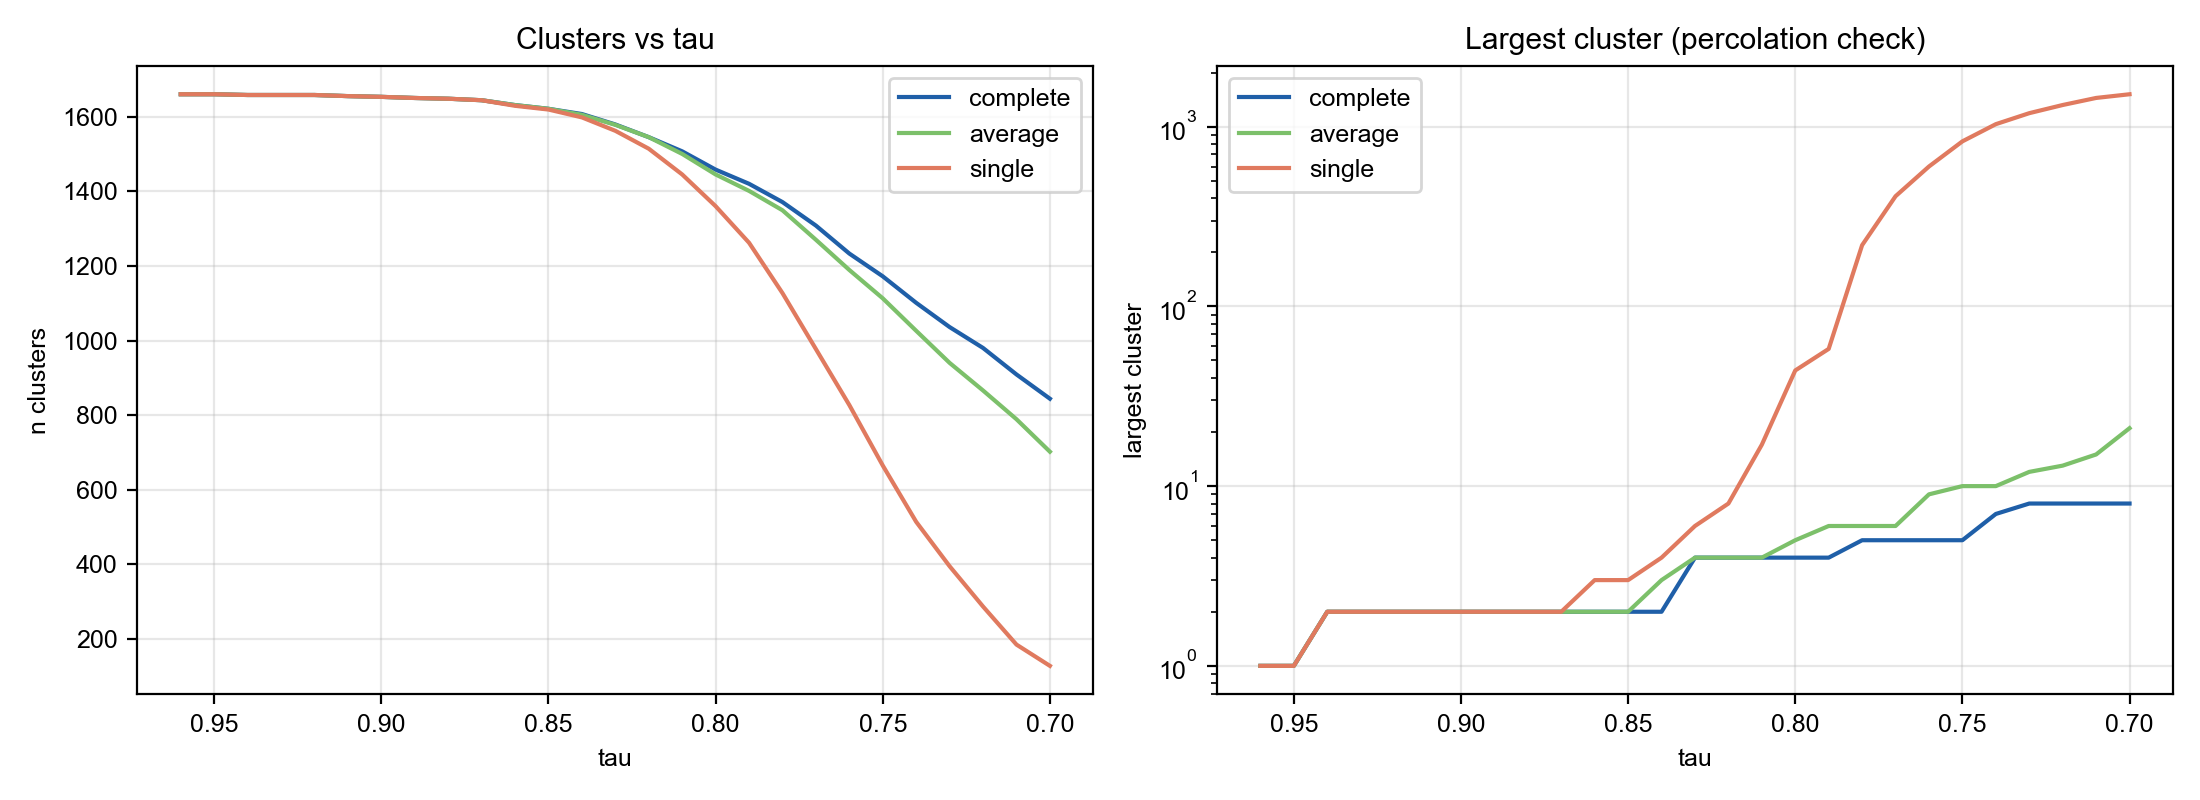
\includegraphics[width=0.95\linewidth]{fig_merge_curve.png}
\caption{$\tau$ 감축 곡선(좌)과 최대 군집 크기(우, log). single linkage의 percolation collapse가 뚜렷하다.}
\end{figure}

\subsection{$\tau$ 감소에 따른 신뢰도의 이중성}

\begin{figure}[htbp]
\centering
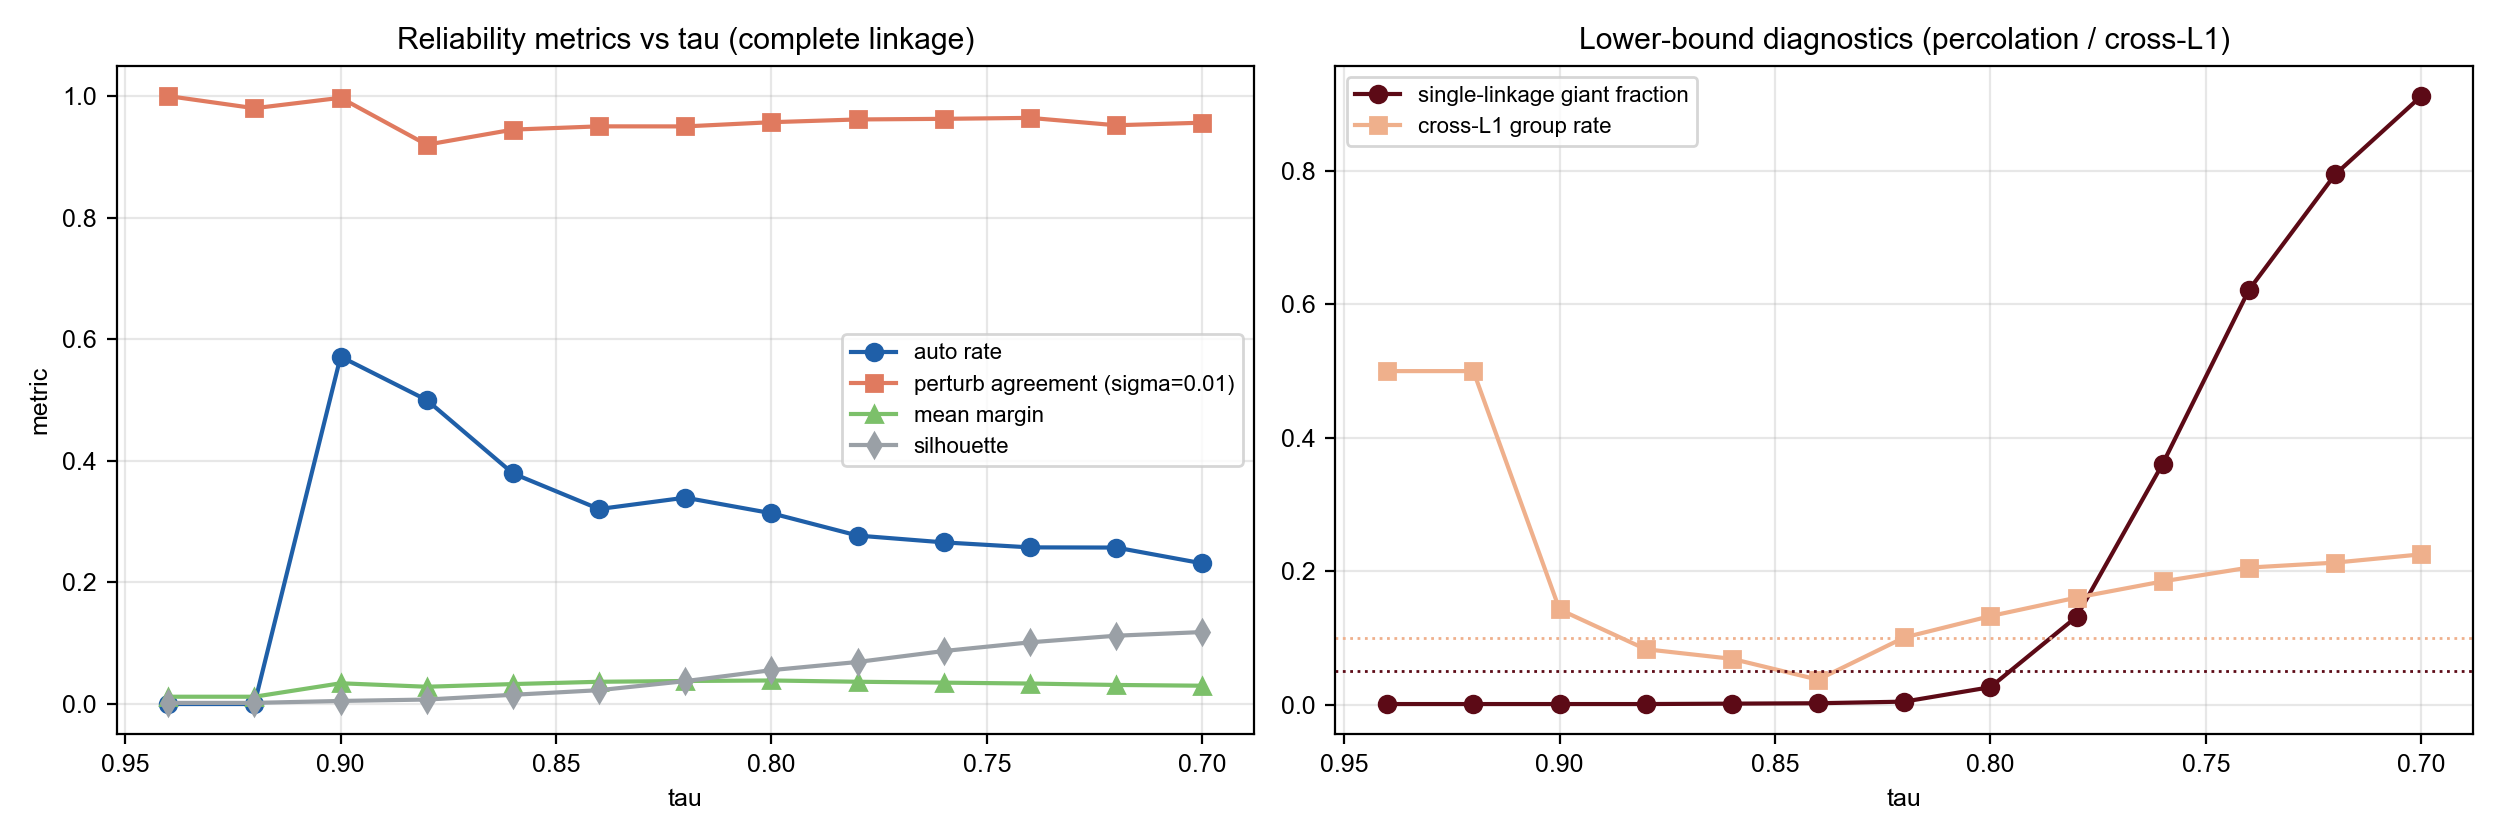
\includegraphics[width=0.95\linewidth]{fig_tau_reliability_sweep.png}
\caption{$\tau$ sweep 신뢰도 지표(좌)와 하한 진단(우).}
\end{figure}

perturbation agreement는 전 구간 $0.94 \sim 0.98$로 안정적이나, auto rate는 $0.67(\tau=0.90) \to 0.22(\tau=0.70)$로 단조 하락하고 cross-L1 혼입률은 0.23까지 상승한다. 즉 기계적 매핑 안정성과 분류학적 정당성이 분리되며, $\tau$ 하강의 비용은 후자에 집중된다. 군집 구조 ARI는 $\sigma=0.01$에서도 세밀 수준($\tau=0.88$)의 소그룹이 0 수준으로 붕괴하여, 2장 규모의 병합 그룹은 임베딩 섭동에 취약함을 보였다. 이는 임계값 단독 병합 확정을 금지하고 전문가 심의를 필수화하는 정량 근거다.

$\tau$ 하한은 세 기준의 최댓값으로 정의된다. single-linkage percolation 임계($\tau_c \approx 0.78$), cross-L1 혼입 10\% 임계, agreement 90\% 임계이다. 실증적으로 운영 병합 하한은 $0.88 \sim 0.90$, 표시용 계층 하한은 $0.78$이며, 권장 step은 $\Delta\tau=0.02$(하한 부근 0.01 세분)이다.

\subsection{신규 카드 L3 매핑의 신뢰도}

$\tau_{op}=0.88$의 병합 그룹 11건에 대해 3종 검증을 적용한 결과, EM은 2 스텝에 수렴($J: 0.831 \to 0.845$), top-1/top-3 containment 100\%, perturbation stability는 $\sigma=0.01$에서 96.0\%, $\sigma=0.05$에서 83.9\%였다(200회 반복). 매핑 자체는 신뢰 가능하나 margin이 $0.002 \sim 0.094$로 얇은 그룹이 있어 개별 확인이 필요하다.

\begin{figure}[htbp]
\centering
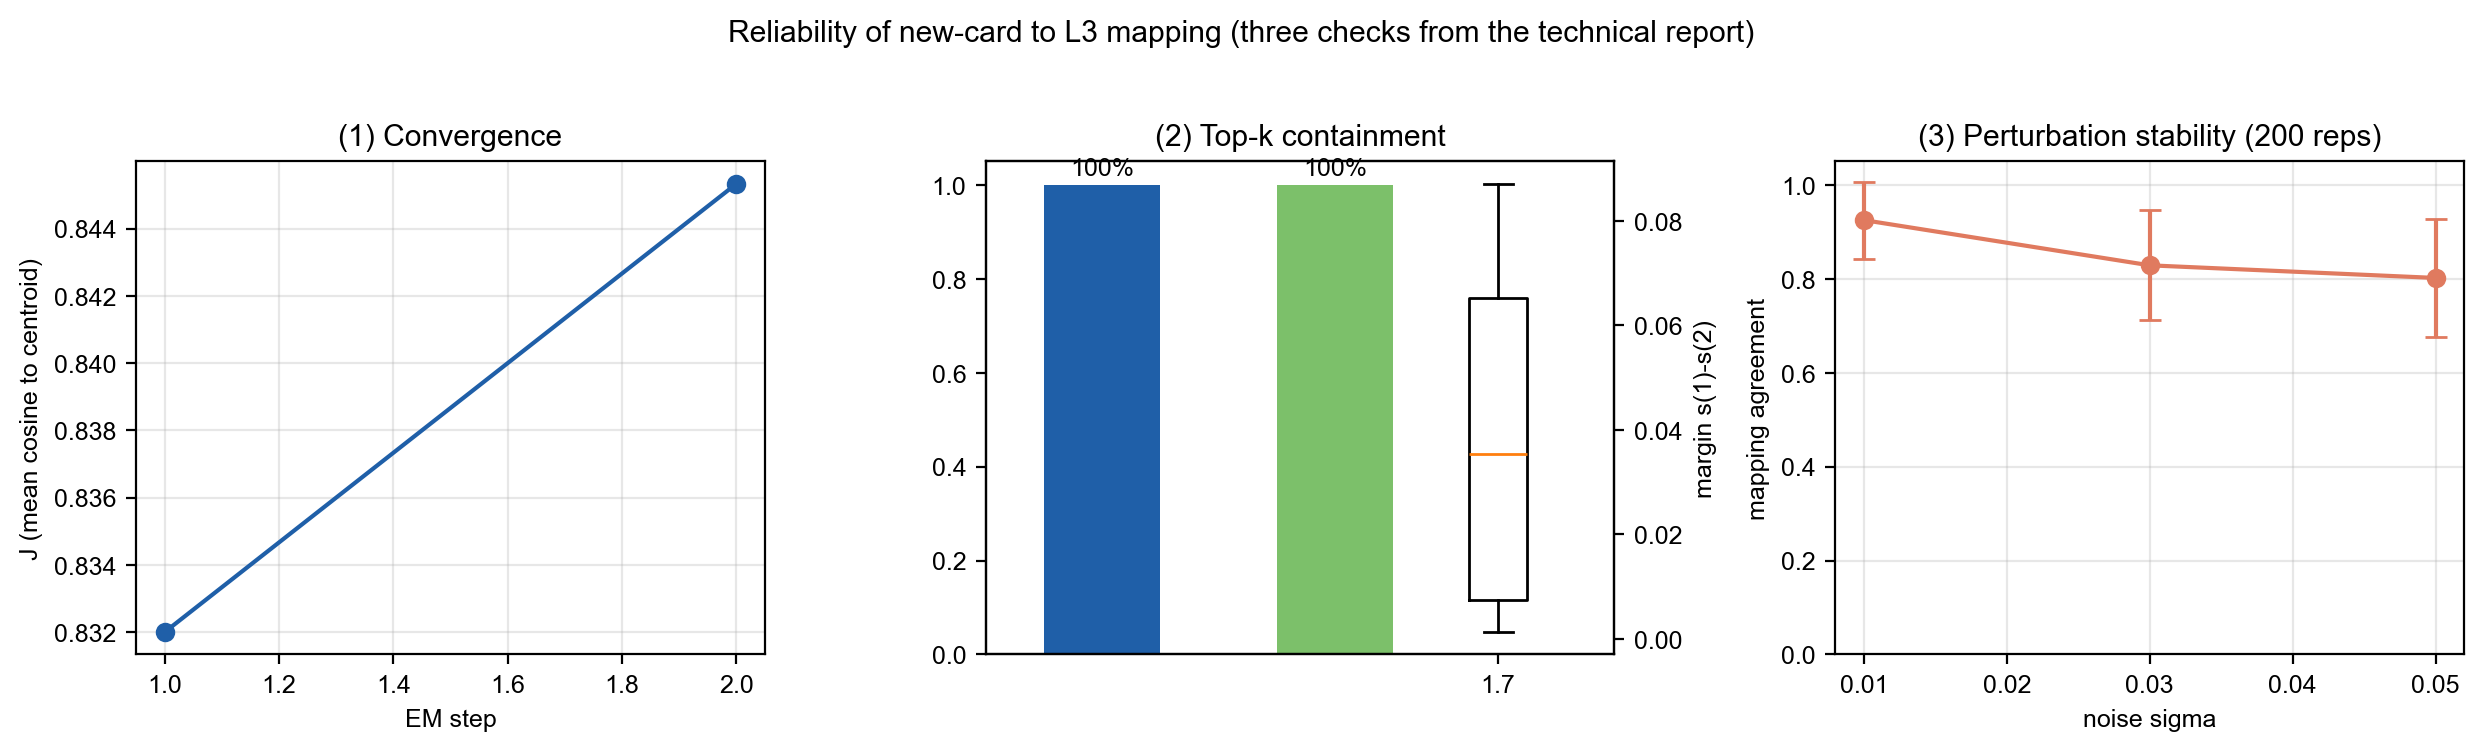
\includegraphics[width=0.95\linewidth]{fig_l3_mapping_reliability.png}
\caption{신규 카드 $\to$ L3 매핑의 3종 신뢰도 검증. (1) EM convergence, (2) top-k containment와 margin, (3) perturbation stability.}
\end{figure}

\subsection{2인 검수 결과와 원천 손상의 발견}

11건의 초안에 대한 검수 결과, 검수자 A는 전 건에서 용어·문체 교정을 제시하였고(``경쟁성''$\to$``이의제기 가능성'', ``전선 AI''$\to$``프론티어 AI'' 등), 검수자 B는 4건을 보류시켰다. 보류 사유 중 2건(g1462, g1458)은 구성 카드의 라벨-정의 불일치, 1건(g81)은 별개 벤치마크 구성개념(명시적 vs 암묵적 위험 거부)의 과병합, 1건(g1582)은 메커니즘 혼합과 L3 오배정이었다. 또한 동일 L3의 허위정보 카드 3장(g520, g1388, g1389)이 실질 중복으로 판정되어 차기 umbrella 통합 대상으로 지정되었다.

\subsection{원천 손상의 전수 검증과 교정}

전수 스크리닝 결과 동일 정의-상이 라벨 손상은 정확히 3쌍 6장이며, 전부 global\_1726 소스의 \texttt{source\_mechanism\_only\_v2.7} 추출 파이프라인에서 발생하였다. 원 소스 문헌 대조 결과는 다음과 같다.

\begin{table}[htbp]
\centering
\small
\caption{원천 손상 3건의 진단과 교정}
\begin{tabular}{p{2.6cm}p{3.4cm}p{3.2cm}p{5.0cm}}
\toprule
카드 & 손상 유형 & 원 소스 & 교정과 병합 판정 환류 \\
\midrule
RAI4-0659 (허위정보 대량생성) & 정의 오복사 (0892의 금융 데이터 정의) & arXiv:2410.23472 GPAI 카탈로그 & 참 정의 복원. g1462 병합 무효. 0659는 허위정보 umbrella로 귀속, 0892는 금융 카드 존치 \\
RAI4-0863 (도덕적 판단 영향) & 정의 오복사 (0870의 금융 GPAI 정의) & arXiv:2410.23472, \S10.3 & 참 정의 복원. g1458 병합 무효. 0863은 가치·상호작용 계열 L3로 분리 재매핑 \\
RAI4-1427/1428 (편향 증폭/유해 응답) & 단일 문장 과분할 & UK Gov Future Risks of Frontier AI, Annex A \S79 & 원 소스가 단일 서술이므로 g1582 병합 정당화(검수자 B 의견을 소스 증거로 번복). L3는 General 브랜치로 재매핑 \\
\bottomrule
\end{tabular}
\end{table}

이 결과는 임베딩 유사도 기반 병합 후보의 일부가 원천 데이터 품질 문제의 산물일 수 있음을 보여준다. 역으로, 병합 파이프라인이 데이터 품질 감사 도구로도 기능함을 시사한다.

\subsection{최종 판정}

교정 환류 후 최종 판정은 다음과 같다. 병합 승인 8건(g1562, g178, g957, g964, g520, g1388, g1389, g1582), 분리 유지 2건(g81은 별개 평가 구성개념, g1462·g1458은 병합 해체 후 각 카드 존치·재매핑), 잔여 검토 1건(g1388의 RAI4-1201 fraud 구성개념 여부). 이번 라운드의 순 감축은 8장이며, 허위정보 umbrella 통합(3~4장 추가 감축)과 HOLD 614장 해소가 차기 라운드로 이관된다.

\section{운영 규칙 확정과 남은 결정}

본 실증으로 확정하는 운영 규칙은 다음과 같다. (1) 병합은 complete linkage만 사용한다. (2) 운영 병합(카드 삭제)은 $\tau \geq 0.88$의 동일 L3 그룹에 한하며, 임계값은 후보 발굴 수단이고 확정은 반드시 2인 검수를 거친다. (3) $\tau \leq 0.82$ 수준은 표시·탐색용 계층으로만 사용한다. (4) 병합 확정 전 구성 카드의 원천 정합성(라벨-정의 일치)을 확인한다. (5) 모든 병합은 \texttt{merged\_into} 계보와 구 ID 매핑을 포함해 날짜 명기 릴리스로만 반영한다.

남은 결정 사항은 (i) 임베딩 정본 확정(ollama 구현체와 웹사이트 근접 네트워크 간 병합 그룹 수가 11 vs 91로 상이), (ii) 허위정보 umbrella 카드의 설계, (iii) HOLD 해소 라운드의 심의 체계, (iv) v2.19 릴리스의 신규 카드 ID 규칙이다.

\section*{산출물 목록}

\texttt{reports/consolidation/simulation/} 하위. dendrogram\_simulation\_1660.\{ipynb, html\} (Task 1--10 실행 기록), embeddings\_bge-m3\_1660.npy, level\_assignments\_complete.csv, dendrogram\_summary.json, merged\_card\_proposals\_tau088.csv, draft\_cards\_for\_review.json, reviewed\_cards\_final.json, merge\_before\_after\_reviewed\_tau088.html (Before/Draft/Reviewed 3단), source\_corruption\_\{screening, corrections\}.json, fig 6종 PNG.

\end{document}
